% Módulo: A12_otimizacao
% Conceito: estudo_monotonia
% Tipo: problema_real_monotonia
% Dificuldade: 2
% Tags: problema_real, otimização, monotonia

\exercicio{
Numa pastelaria, a quantidade de massa (em kg) foi registada.

\begin{center}
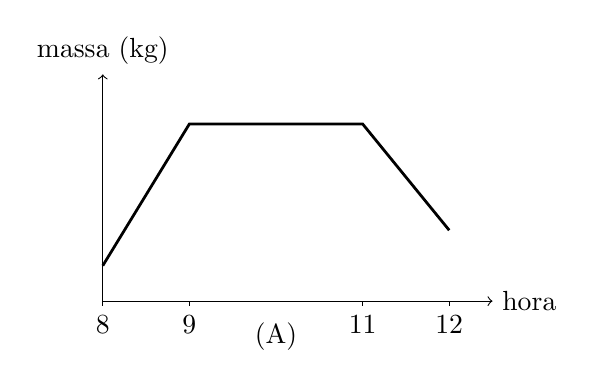
\begin{tikzpicture}[x=1.1cm,y=0.9cm]
    \draw[->] (0,0) -- (4.5,0) node[right] {hora};
    \draw[->] (0,0) -- (0,3.2) node[above] {massa (kg)};
    \draw[line width=1pt] (0,0.5) -- (1,2.5) -- (3,2.5) -- (4,1.0);
    \foreach \x/\lab in {0/8,1/9,3/11,4/12} \draw (\x,0) -- (\x,-0.07) node[below] {\lab};
    \node at (2,-0.5) {(A)};
\end{tikzpicture}
\end{center}

Qual dos gráficos melhor representa?
}

\subexercicio{Indique a letra do gráfico.}
\subexercicio{Justifique a sua escolha.}
